% ============================================================
%  PROBLEM 4 — worked example
%  Shows: subequations, \align, \underbrace annotation, a boxed result
%         and an unnumbered display equation.
% ============================================================

\section*{Problem 4}
\phantomsection
\addcontentsline{toc}{section}{Problem 4}

The task is to integrate a three-dimensional continuous dynamical system, to
locate its fixed points analytically, and to comment on the trajectory that
results. The system is the one introduced by Rössler \cite{rossler1976} as the
simplest continuous system exhibiting chaos:

\begin{subequations}
	\label{eq:rossler}
	\begin{align}
		\dot{x} &= -y - z          \label{eq:rossler_x} \\
		\dot{y} &= x + ay          \label{eq:rossler_y} \\
		\dot{z} &= b + z(x - c)    \label{eq:rossler_z}
	\end{align}
\end{subequations}

with the standard parameter set $a = b = 0.2$ and $c = 5.7$. Two of the three
equations are linear; all of the nonlinearity sits in the single product term
of \cref{eq:rossler_z}:

\begin{equation} \label{eq:nonlinear}
	\dot{z} = \underbrace{b}_{\text{constant drive}}
	         + \underbrace{zx}_{\text{the only nonlinear term}}
	         - \underbrace{cz}_{\text{linear decay}}
\end{equation}

\Cref{eq:nonlinear} explains the shape of the attractor before any integration
is done. While $x < c$ the $z$ component decays and the trajectory stays in a
nearly planar spiral driven by \cref{eq:rossler_x} and \cref{eq:rossler_y};
once the spiral grows far enough that $x > c$, the product term turns positive,
$z$ grows sharply, and the trajectory is lifted out of the plane before falling
back into the spiral.

The fixed points follow from setting all three derivatives to zero. From
\cref{eq:rossler_x} and \cref{eq:rossler_y},

\begin{equation*}
	y = -\frac{x}{a} \; \; \; \text{, } \; \; \; z = \frac{x}{a}
\end{equation*}

and substituting both into \cref{eq:rossler_z} gives the quadratic
$x^2 - cx + ab = 0$, so that

\begin{equation} \label{eq:fixed}
	\boxed{
		x_\pm = \frac{c \pm \sqrt{c^2 - 4ab}}{2}
		\; \; \; \text{, } \; \; \;
		y_\pm = -\frac{x_\pm}{a}
		\; \; \; \text{, } \; \; \;
		z_\pm = \frac{x_\pm}{a}
	}
\end{equation}

With the standard parameters, the discriminant in \cref{eq:fixed} is
$c^2 - 4ab = 32.33$, giving two real fixed points: one at
$(0.0070,\, -0.0351,\, 0.0351)$ near the origin, around which the spiral
winds, and one far out at $(5.6930,\, -28.4649,\, 28.4649)$. Both are unstable
\cite{strogatz}, which is what keeps the trajectory circulating instead of
settling.

\Cref{eq:rossler} was integrated with a fixed-step fourth-order Runge–Kutta
scheme, $\Delta t = 0.005$, over $t \in [0, 500]$, discarding the first $10\%$
as transient. The step size matters more than the total time: with
$\Delta t$ an order of magnitude larger the sharp excursion described by
\cref{eq:nonlinear} is under-resolved and the trajectory drifts off the
attractor entirely. The result is shown in \cref{fig:rossler}, and the
integrator itself is listed in the appendix.

\begin{figure}[htbp]
	\centering
	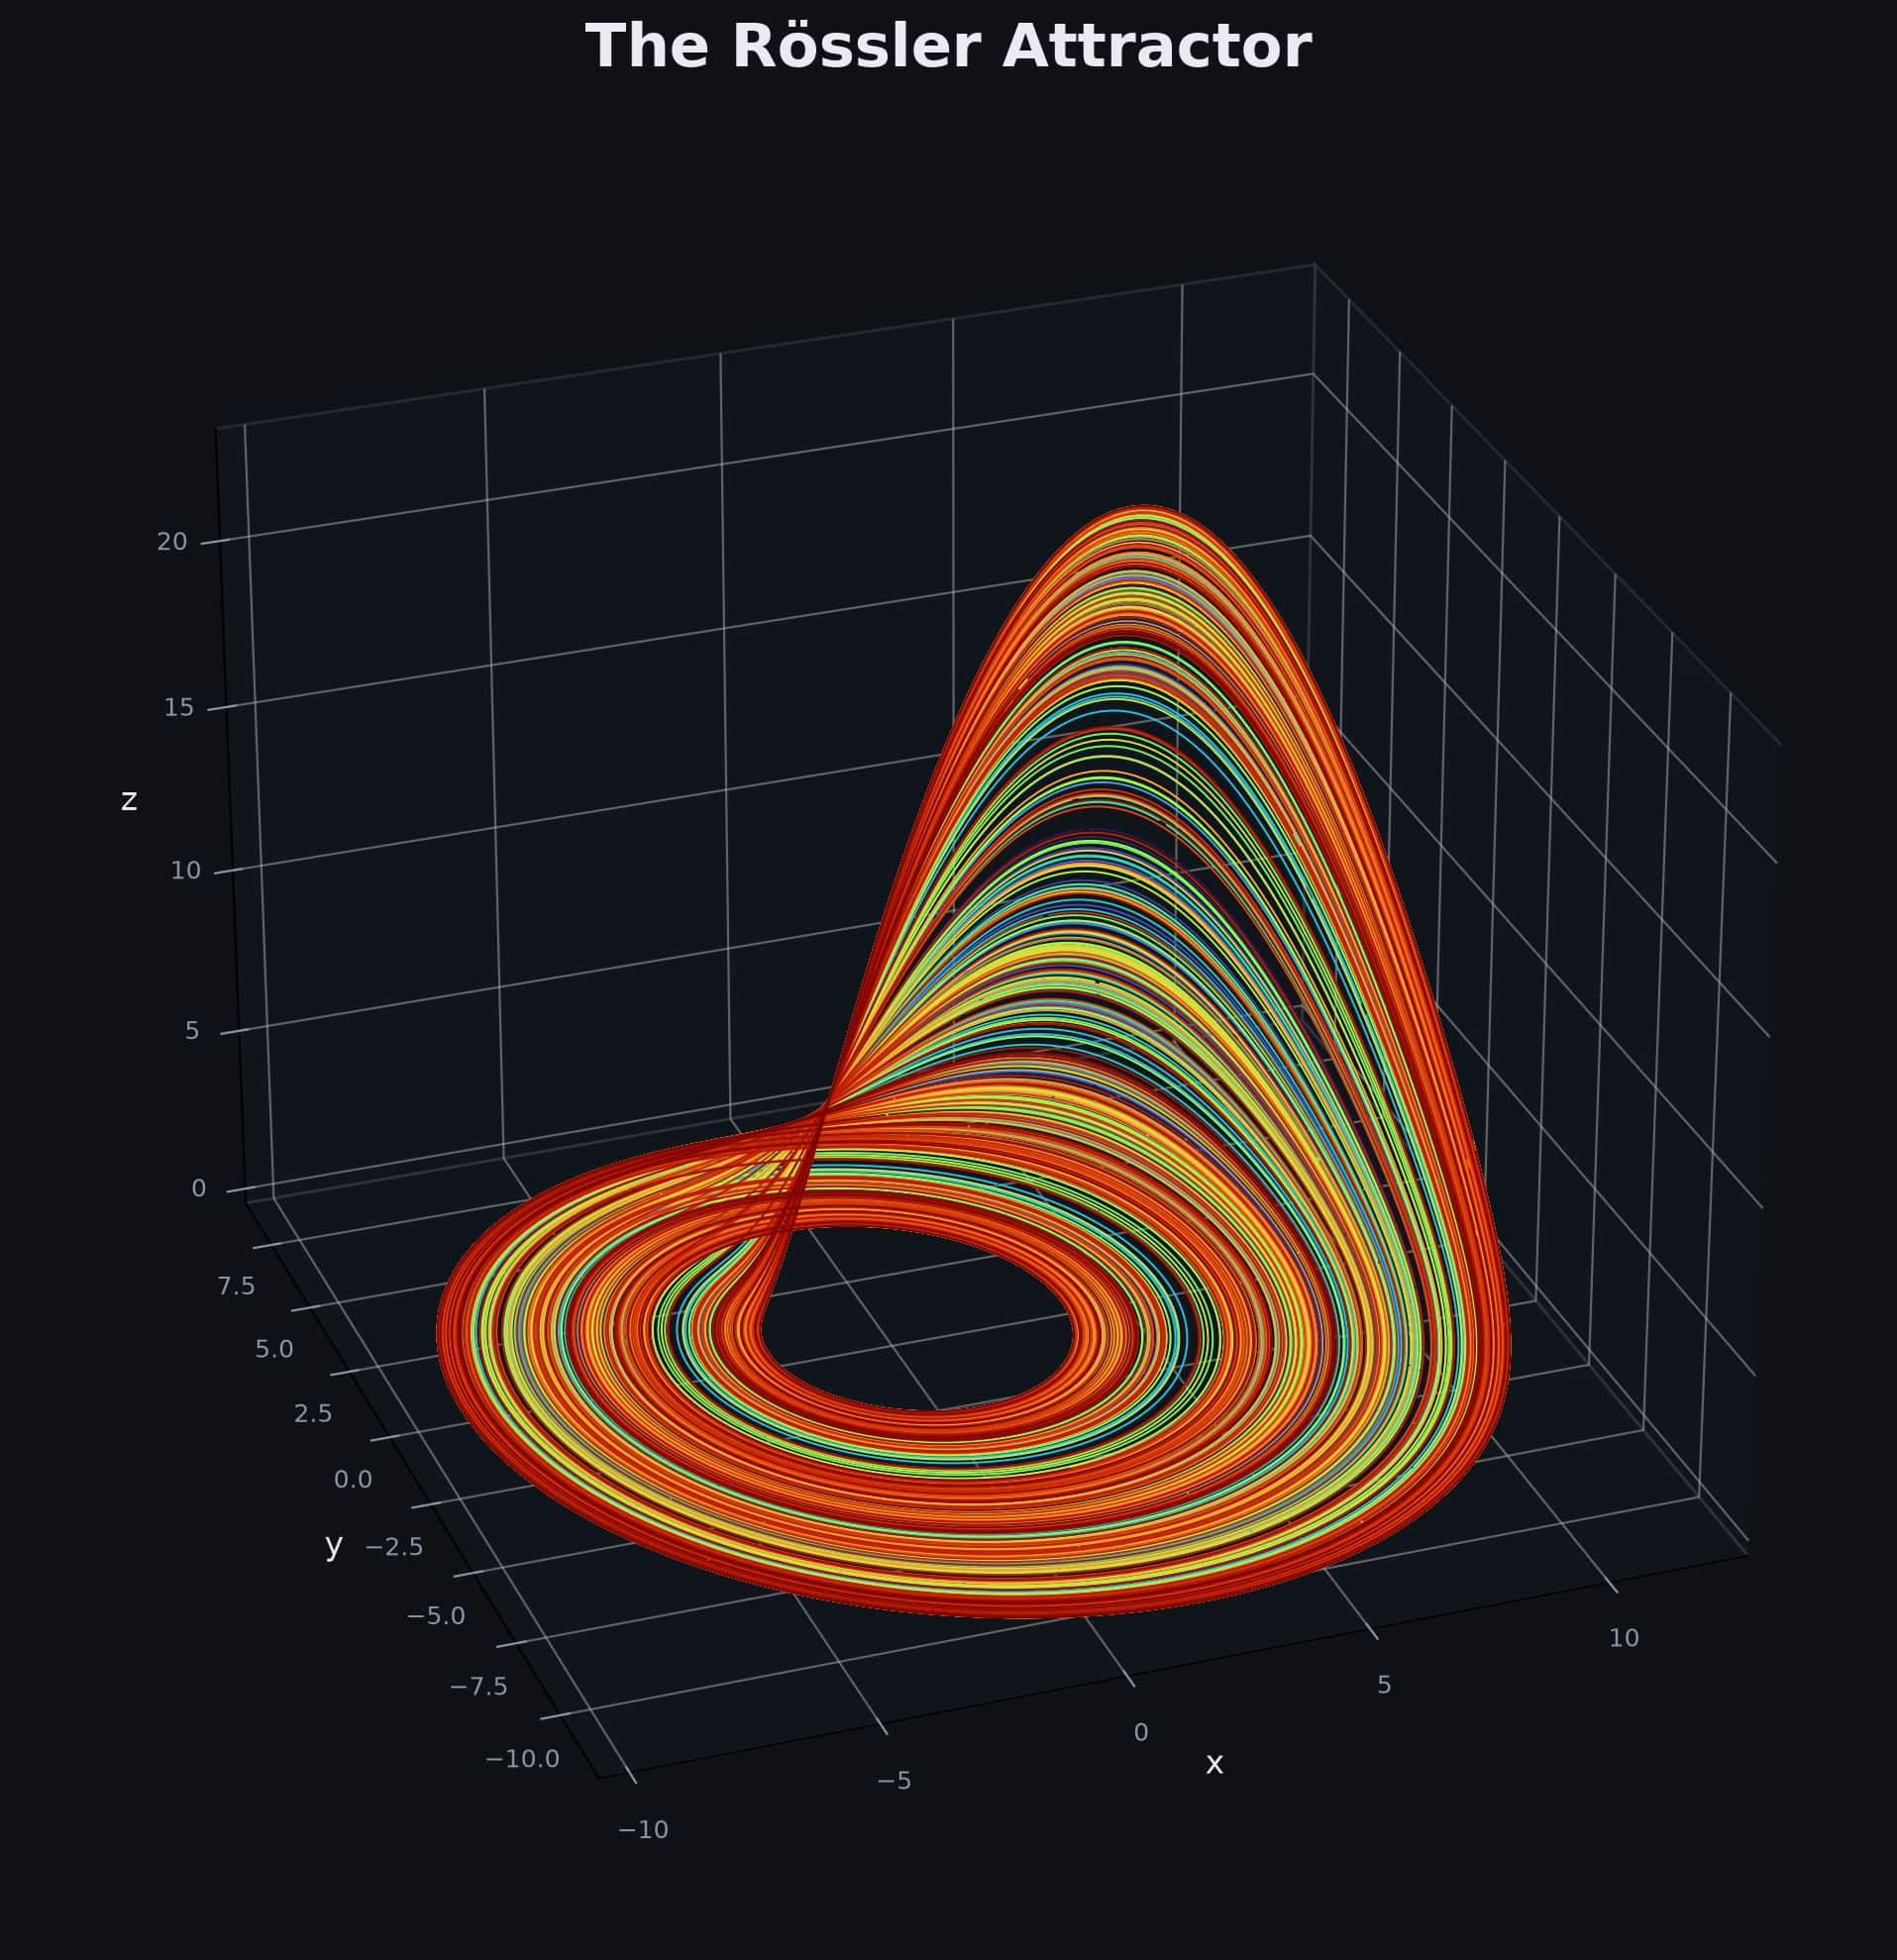
\includegraphics[width=0.80\linewidth]{graphs/rossler}
	\caption{A single trajectory of \cref{eq:rossler} with $a = b = 0.2$,
	$c = 5.7$, coloured by time. The flat spiral is the regime where
	$x < c$ in \cref{eq:nonlinear}; the fold rising out of it is where the
	nonlinear term takes over.}
	\label{fig:rossler}
\end{figure}

Two things are worth noting from \cref{fig:rossler}. First, the trajectory
never closes: it is bounded but aperiodic, and no matter how long it is
integrated it does not repeat. Second, the band is thin but not
two-dimensional — successive sheets lie arbitrarily close together without
touching, which is the geometric signature of the stretching-and-folding
mechanism that \cref{eq:nonlinear} implements.

\clearpage
